\section{Warstwy oraz ich rysowanie}
\label{sec:warstwy_oraz_ich_rysowanie}

Podstawowym założeniem jest przedstawienie komórki na schemacie jako \textit{GameObject} zawierający dwuwymiarowe,
kwadratowe sprite'y,
stąd cały obszar roboczy jest przedstawiony jako siatka.
Komórki dla danej warstwy leżą na jednej płaszczyźnie XY, a~kolejne warstwy są przesunięte w~osi Z,
co~daje efekt nakładania się na siebie.
Ponieważ warstwy oraz ich rysowanie są kluczowymi elementami, definiującymi działanie reszty programu,
a~zarazem stanowią najbardziej obciążającą komputer część projektu,
należało rozpatrzyć kilka rozwiązań, które można zaimplementować do przedstawiania rysowanego schematu,
pod kątem optymalizacja oraz współdziałania z~resztą programu.\\

\indent Jednym z~najprostszych sposobów do zapisania danych warstwy to tablica dwuwymiarowa,
gdzie każdy element tablicy odpowiada jednemu kwadratowi na siatce.
%Jeszcze lepiej podzielić taką tablicę na kilka mniejszych oraz przenieść ją do jednego wymiaru.
Dodatkowo w~celu optymalizacji taką tablicę można podzielić na kilka mniejszych,
odpowiedzialnych za różne obszary, a~także zamienić je na tablice jednowymiarowe.
Rozwiązanie takie pozwala na optymalniejsze zarządzanie pamięcią,
ponieważ całą warstwę można zapisać jako tablice bitów,
gdzie każdy bit odpowiada jednej komórce i~\texttt{1} oznacza,
że~jest zajęta a~\textt{0} -- wolna.
W~połączeniu z~tym rozwiązaniem można wyróżnić dwie metody rysowania warstw:

\begin{citemize}
    \item Rysowanie co~modyfikację całej warstwy od nowa -- w~tej metodzie cała warstwa jest rysowana od nowa po każdej modyfikacji,
    nie ma tu potrzeby sprawdzania każdego kwadratu czy jest zajęty, pozwala to również na pośrednie modyfikowanie narysowanej warstwy,
    bez potrzeby posiadania referencji do obiektów na scenie.
    Wadą jest jednak rysowanie całej warstwy po każdej modyfikacji,
    co~przy dużym obszarze roboczym i~dużej ilości już narysowanych elementów wpłynie negatywnie na optymalizację.
    \item Rysowanie tylko zmienionych kwadratów -- w~tej metodzie komórki są rysowane tylko wtedy, gdy nie są puste,
    co~w~ogólnym rozrachunku jest szybsze, jednak wymaga sprawdzania każdej komórki czy nie jest zajęta,
    oraz w~celu modyfikacji już istniejących elementów, potrzebne jest posiadanie referencji do GO na scenie.
\end{citemize}

%rysowanie co~zmianę całości od nowa, dzięki czemu nie trzeba sprawdzać każdego kwadratu czy już jest zajęty,
%oraz rysowanie tylko zmienionych kwadratów, co~w~ogólnym rozrachunku jest szybsze,
%natomiast wymaga sprawdzanie każdej komórki czy nie jest zajęta,
%aby nie doszło do sytuacji, gdzie sprite'y się nakładają.
Niestety powyższe rozwiązania wymagają ciągłego iterowania po całej tablicy nawet przy modyfikacji jednego elementu
i~albo dodatkowego przetrzymywania referencji, albo ciężkiego obliczeniowo rysowania całej warstwy od nowa.
W~związku z~tym wybrano inne rozwiązanie, polegające na wykorzystaniu systemu fizyki w~silniku Unity,
który pozwala na wykrywanie kolizji pomiędzy obiektami.
Daje to możliwość na niezależne wykrywanie komórek bez potrzeby referencji do nich i~ich położenia,
znacząco upraszczając zarządzanie nimi oraz proces rysowania.
W~tym celu do obiektu komórki prócz komponentu \texttt{SpriteRenderer} dodano komponent \texttt{BoxCollider},
dzięki czemu obiekt ten może być wykrywany przez system fizyki.\\
\indent Kolejnym sposobem na optymalizację jest wykorzystanie puli obiektów.
Ponieważ w~wielu przypadkach potrzebne będzie stworzenie wielu komórek naraz, co~jest kosztowne obliczeniowo,
w~trakcie działania programu, co~klatkę tworzy się jedynie kilka nieaktywnych obiektów,
które są następnie przechowywane w~puli.
Gdy potrzebny jest nowy obiekt, pobiera się go z~puli i~aktywuje, gdy nie jest już potrzebny,
jest on dezaktywowany i~przenoszony z~powrotem do puli.
W~przypadku gdy w~puli brakuje obiektów, tworzy ona nowe i~zwraca je bezpośrednio w~metodzie pobierającej obiekt.
Do implementacji tego mechanizmu stworzono komponent \texttt{CellsPool},
posiadający listę struktur \texttt{PoolData} dla każdej z~warstw.
Struktura ta przechowuje informację o tym, dla jakiej warstwy jest pulą oraz samą pulę obiektów.
Do przetrzymywania tworzonych instancji wykorzystano klasę \texttt{Queue},
jest to struktura danych FIFO (ang. \textit{First In, First Out}),
która pozwala na dodawanie elementów na koniec kolejki oraz usuwanie z~jej początku.
%Aby uporządkować w~hierarchii w~edytorze wszystkie tworzone w~puli obiekty,
%jako swojego rodzica mają ustawiony obiekt \texttt{CellsPool}\\
Wszystkie obiekty w~puli mają ustawionego rodzica \texttt{CellsPool} w~celu uporządkowania hierarchii w~edytorze.\\
\indent Do definiowania warstw stworzono \texttt{ScriptableObject}, \texttt{LayerConfig}.
Zawiera on informacje o nazwie warstwy, jej kolejności na schemacie, jaki sprite ma być rysowany, kolor,
zasady projektowania (minimalna odległość między niesąsiadującymi komórkami, minimalna szerokość)
oraz maksymalną wielkość puli komórek.
Dzięki temu można w~łatwy sposób tworzyć nowe warstwy, a~także modyfikować definicje już istniejących.
Nazwa warstwy jest również wykorzystywana jako tag dla komórek, co~pozwala na późniejsze ich rozróżnienie.
Dodatkowo \texttt{LayerConfig} jest używany jako klucz do identyfikacji warstwy w~innych komponentach.
Przykład takiej konfiguracji przedstawiono na rys.~\ref{fig:layer_config}.

\begin{figure}[h]
    \centering
    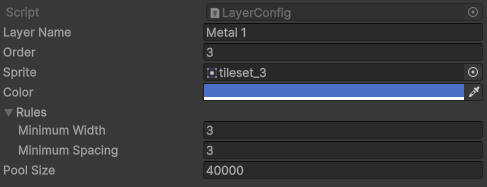
\includegraphics[width=.9\textwidth]{chapters/chapter4/rys/layer_config}
    \caption[Przykładowe okno konfiguracji warstwy \textit{Metal 1}.]
    {Przykładowe okno konfiguracji warstwy \textit{Metal 1}, źródło: opracowanie własne.}
    \label{fig:layer_config}
\end{figure}

\indent W~trakcie działania programu wszystkie narysowane komórki danej warstwy
są przechowywane w~komponencie \texttt{LayerHolder} jako lista obiektów \texttt{GameObject}.
Komponent ten jest także w~głównej mierze odpowiedzialny za rysowanie
i~usuwanie pojedynczych komórek poprzez metody \texttt{NewCell} oraz \texttt{ReturnCell}.
a~także umożliwia dostęp do wszystkich komórek danej warstwy.
Inicjalizacją \texttt{LayerHolder} zajmuje się \texttt{LayersManager}, podczas startu programu.
Z~jego głównych funkcji można wymienić:

\begin{citemize}
    \item Tworzenie warstw na podstawie konfiguracji z~\texttt{LayerConfig},
    \item Przechowywanie referencji do wszystkich warstw,
    \item Wybór oraz zwracanie obecnie rysowanej warstwy,
    \item Włączanie i~wyłączanie warstw (gdy warstwa jest wyłączona, nie można na niej rysować oraz jest niewykrywana),
    \item Pośredniczenie przy zwracaniu komórek do puli.
\end{citemize}


Aby zdefiniowane w~plikach konfiguracyjnych warstwy były użyte w~programie,
należało je przypisać do \texttt{LayersManager} w~inspektorze Unity w~obiekcie \textit{Layers} tak jak na rys.~\ref{fig:layers}.
Na tym samym obiekcie znajduje się także \texttt{CellsPool},
natomiast reszta elementów jest doładowywana w~trakcie działania programu.

\newpage % TODO: check this if something changes

\begin{figure}[h]
    \centering
    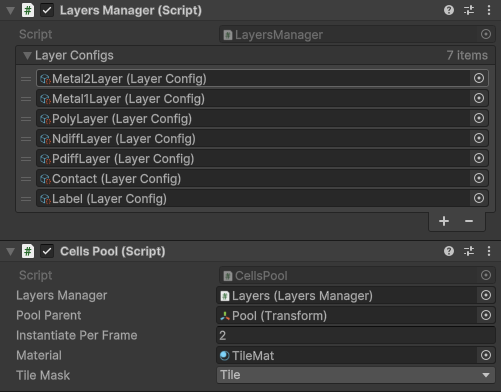
\includegraphics[width=.9\textwidth]{chapters/chapter4/rys/layers}
    \caption[Okno konfiguracji warstw w~obiekcie \textit{Layers}.]
    {Okno konfiguracji warstw w~obiekcie \textit{Layers}, źródło: opracowanie własne.}
    \label{fig:layers}
\end{figure}

Ze względu na istotność komponentu \texttt{LayersManager},
zdecydowano się na zastosowanie wzorca projektowego \textit{Singleton}~\cite{unity_csharp},
dzięki czemu jest on dostępny z~każdego miejsca w~programie
oraz implikuje posiadanie tylko jednej instancji tego obiektu w~trakcie działania programu.
W~przypadku Unity, ze względu na to, że~klasą bazową komponentów jest \texttt{MonoBehaviour},
należało zaimplementować wzorzec poprzez opracowanie klasy \texttt{MonoSingleton},
której kod przedstawiono na listingu~\ref{lst:monosingleton}.

\begin{lstlisting}[language={C},label=lst:monosingleton,caption={Klasa \texttt{MonoSingleton}}]
public class MonoSingleton<T> : MonoBehaviour where T : Component {
    public static T Instance => _instance;
    private static T _instance;
    protected void Awake() {
        if (_instance != null && _instance != this as T)
            throw new Exception($"Singleton already exists! : {_instance.name}");
        _instance = this as T;
    }
}
\end{lstlisting}
